\documentclass{beamer}
\usepackage[utf8]{inputenc}
\usepackage[T1]{fontenc}
\usepackage[french]{babel}

\usepackage[export]{adjustbox}
\usepackage{array}
\usepackage{color, colortbl}

\usepackage{graphicx}

\usetheme{JuanLesPins}
\setbeamercolor{structure}{fg=arkred, bg=arkbrown}

% colors
\definecolor{gray73}{gray}{0.73}
\definecolor{arkred}{rgb}{0.592, 0.145, 0.168}
\definecolor{arkbrown}{rgb}{0.239,0.235,0.204}

\graphicspath{{../images/}}

\title{Rapport de stage \\Master 2 -- Fiabilité et Sécurité Informatique}
\subtitle{Conception \&  d\'eveloppement syst\`eme de backup chiffr\'e et
incr\'emental en C/C++}
\author{Ludovic Lubeigt}
\institute{Aix-Marseille Universit\'e}
\date{18 septembre 2015}

\AtBeginSubsection[]
{
  \begin{frame}
  \frametitle{Sommaire}
  \tableofcontents[currentsection, currentsubsection, hideothersubsection]
  \end{frame} 
}

\AtBeginSection[]
{
  \begin{frame}
   \frametitle{Sommaire}
   \tableofcontents[currentsection, hideothersubsection]
  \end{frame}
}

\begin{document}
\begin{frame}
 \titlepage
\end{frame}

\begin{frame}
 \frametitle{Sommaire}
 \tableofcontents
\end{frame}

\section{Arksens}
\subsection{Pr\'esentation de l'entreprise}
\begin{frame}
 \frametitle{Arksens}
 \framesubtitle{Pr\'esentation de l'entreprise}
 \begin{minipage}{0.49\textwidth}
  \begin{itemize}
    \item Une pr\'esence sur 3 continents
    \item 6 produits
    \item 3 offres clouds
  \end{itemize}
 \end{minipage}
 \begin{minipage}{0.49\textwidth}
  \begin{figure}[h!]
    \centering
    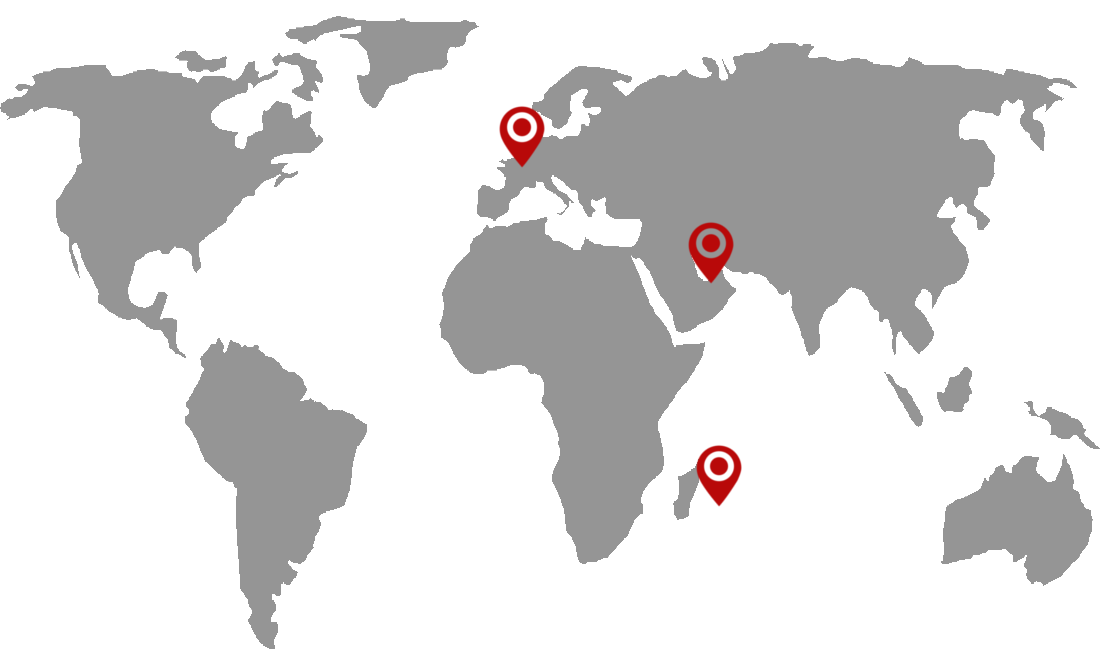
\includegraphics[scale=0.13]{map_arksens.png}
    \caption{O\`u trouver Arksens ?}
  \end{figure}
 \end{minipage}
\end{frame}

\begin{frame}
  \frametitle{Pr\'esentation de l'entreprise}
  \framesubtitle{Les produits et Services}
  \begin{table}[h!]
    \centering
    \def\arraystretch{1.5}
    \setlength{\fboxsep}{13pt} % padding
    \setlength{\fboxrule}{0pt} % frame
    \begin{tabular}{cc}
      \arrayrulecolor{gray73}
      
\includegraphics[width=3cm, fbox]{produits/mail.png} & 
      
\includegraphics[width=3cm, fbox]{produits/whisper.png}\\
      \hline
      
\includegraphics[width=3cm, fbox]{produits/backup.png} &
      
\includegraphics[width=3cm, fbox]{produits/gateway.png}\\
      \hline
      
\includegraphics[width=3cm, fbox]{produits/endpoint.png} &
      
\includegraphics[width=3cm, fbox]{produits/nomad.png}\\
    \end{tabular}
    \caption{Produits et solutions par \textit{Arksens}}
  \end{table}
\end{frame}

\subsection{\^Ile Maurice}
\begin{frame}
  \frametitle{Pr\'esentation de l'entreprise}
  \framesubtitle{\^Ile Maurice}
  \begin{minipage}{0.49\linewidth}
    \begin{itemize}
     \item Recherche et d\'eveloppement
     \item Jusqu'\`a 8 employ\'es + des commerciaux et le PDG
     \item Importante restructuration
    \end{itemize}
  \end{minipage}
  \begin{minipage}{0.49\linewidth}
    \begin{figure}[h!]
      \centering
      \includegraphics[scale=0.23]{beau_plan_soir.jpg}
      \caption{Beau Plan Business Park}
    \end{figure}
  \end{minipage}
\end{frame}

\section{Sujet de stage}
\begin{frame}
 \frametitle{Sujet de stage}
 \begin{itemize}
  \item Conception et d\'eveloppement d'un syst\`eme de sauvegarde 
  chiffr\'e et incr\'emental
  \item Chiffrement local
  \item Multi-plate-forme
 \end{itemize}
\end{frame}

\section{D\'eroulement du stage}
\begin{frame}
 \frametitle{D\'eroulement du stage}
 Trois grandes phases
 \begin{itemize}
  \item Recherche
  \item Conception
  \item D\'eveloppement
 \end{itemize}
\end{frame}

\subsection{Recherche et r\'eflexions}
\begin{frame}
 \frametitle{Recherche et r\'eflexions}
 \framesubtitle{Recherche}
 Des d\'efinitions...
 \begin{itemize}
  \item Backup incr\'emental
  \item Backup diff\'erentiel
  \item Transchiffrement\\[0.51cm]
 \end{itemize}
 
 Et des logiciels...
 \begin{itemize}
  \item Syncthing
  \item rsync
 \end{itemize}
\end{frame}

\begin{frame}
 \frametitle{Recherche et r\'eflexions}
 \framesubtitle{R\'eflexions}
 \begin{itemize}
  \item Chiffrement homomorphique
  \begin{itemize}
   \item Domaine de recherche
   \item Pas utilisable dans des applications aujourd'hui
  \end{itemize}
  \item rsync revisit\'e
  \begin{itemize}
   \item Une base commune avec une fen\^etre parcourant le fichier...
   \item ... mais une importante diff\'erence avec la taille de la fen\^etre
   variant
   \item Un prototype pour valider l'algorithme
  \end{itemize}
 \end{itemize}
\end{frame}

\subsection{Conception}
\begin{frame}
 \frametitle{Conception}
 \framesubtitle{Un programme modulaire}
  \begin{figure}[h!]
    \centering
    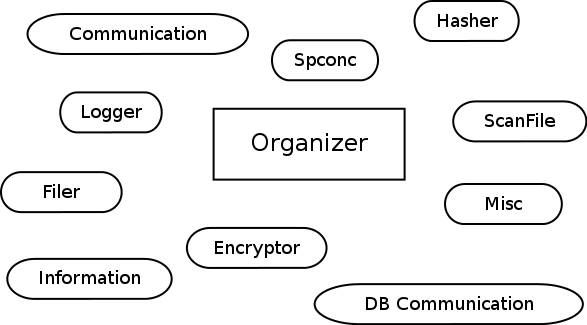
\includegraphics[scale=0.42]{softwareDesign/overviewModule.png}
    \caption{Vue d'ensemble des modules}
  \end{figure}
\end{frame}

\begin{frame}
 \frametitle{Conception}
 \framesubtitle{Interaction entre modules}
 \begin{itemize}
  \item Solution faite \flqq maison\frqq
  \item Design pattern
  \begin{itemize}
   \item Observer
   \item Event notifier
  \end{itemize}
 \end{itemize}
\end{frame}

\begin{frame}
 \frametitle{Interaction entre modules}
 \framesubtitle{Event Notifier}
  \begin{figure}
    \centering
    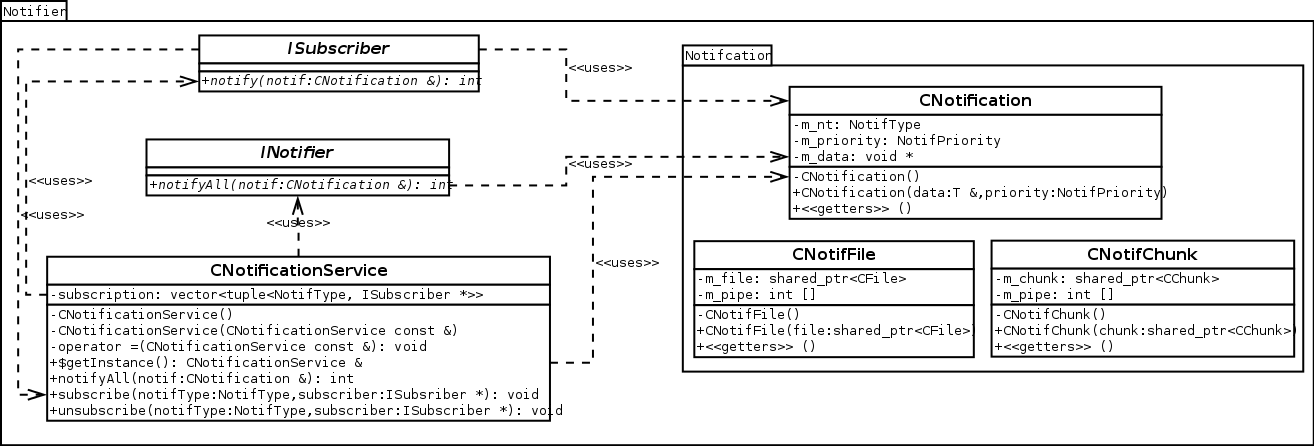
\includegraphics[width=10cm]{softwareDesign/classDiagramNotif.png}
    \caption{Diagramme de classe --- notifications}
  \end{figure}
\end{frame}

\begin{frame}
 \frametitle{Interaction entre modules}
 \framesubtitle{Premi\`ere sauvegarde}
  \begin{figure}
    \centering
    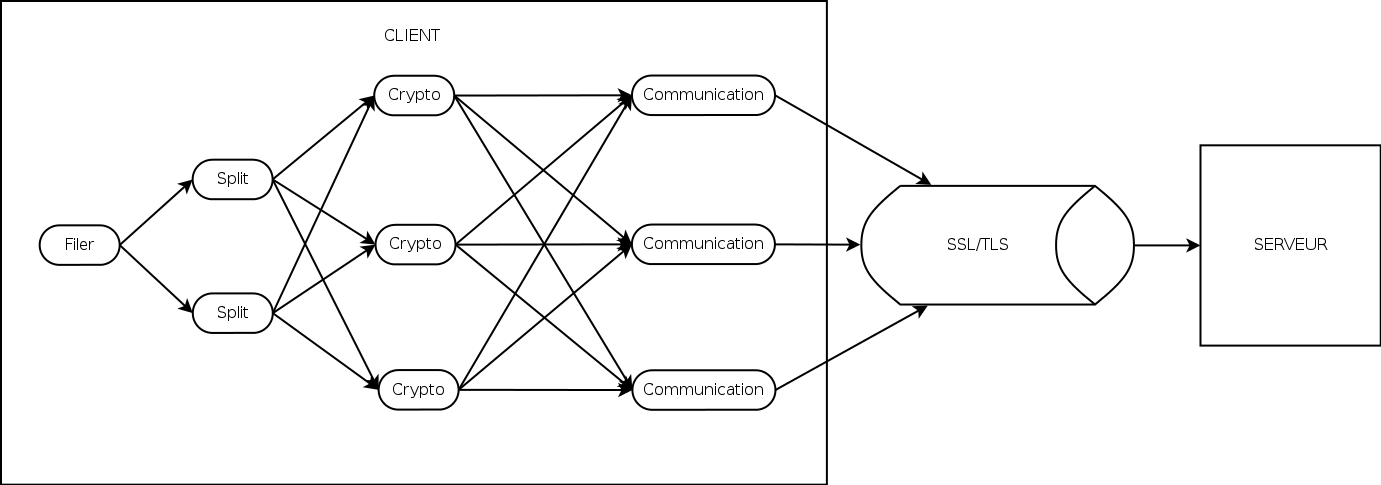
\includegraphics[width=10cm]{softwareDesign/moduleInteraction.png}
    \caption{Fonctionnement lors d'une premi\`ere sauvegarde}
  \end{figure}
\end{frame}

\begin{frame}
 \frametitle{Conception}
 \framesubtitle{Base de donn\'ees}
 \begin{itemize}
  \item Sauvegarder les m\'eta-donn\'ees de tous les fichiers
  \item Sur le serveur
  \begin{itemize}
   \item Garder une trace de toute les sauvegardes
   \item Restaurer un fichier \`a partir de n'importe quelle sauvegarde
  \end{itemize}
  \item Sur le client
  \begin{itemize}
   \item Garder une trace de la derni\`ere sauvegarde
   \item Gagner de temps
   \item \'Economiser de la bande passante
  \end{itemize}
 \end{itemize}
\end{frame}

\begin{frame}
 \frametitle{Base de donn\'ees}
 \framesubtitle{SQL vs NoSQL}
 \begin{table}[h!]
  \def\arraystretch{1.5}
  \setlength{\fboxsep}{13pt} % padding
  \setlength{\fboxrule}{0pt} % frame
  \begin{tabular}{m{2cm}m{4cm}m{4cm}}
   \rowcolor{arkred} 
    \arrayrulecolor{gray73}\hline
    & \color{white} \textbf{\textit{SQL}} &
    \color{white} \textbf{\textit{NoSQL}}\\
    Stockage des donn\'ees & Mod\`ele relationnel & Variable : documents,
    cl\'e-valeur, graphe, etc.\\
    \hline
    Sch\'ema et flexibilit\'e & Sch\'ema fixe & Sch\'ema dynamiques\\
    \hline
    Adaptabilit\'e & \'Evolutivit\'e verticale & \'Evolutivit\'e horizontale\\
    \hline
    Propri\'et\'es ACID\footnote{Atomicit\'e, Coh\'erence, Isolation,
    Durabilit\'e} & Oui & Pas n\'ecessairement\\
  \end{tabular}
  \caption{\label{tabSQLNoSQL} Tableau comparatif \textit{SQL} et
  \textit{NoSQl}}
\end{table}
\end{frame}

\begin{frame}
 \frametitle{Conception}
 \framesubtitle{Stockage des donn\'ees}
  \begin{figure}
    \centering
    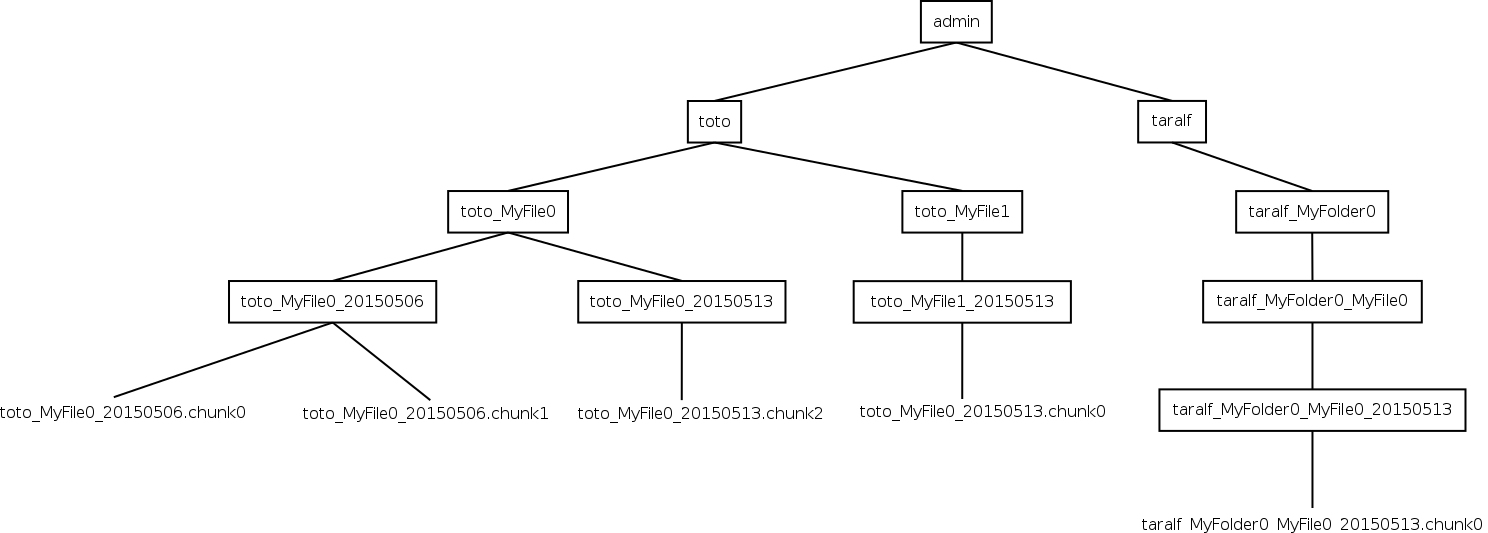
\includegraphics[width=10cm]{softwareDesign/fileSystemServer.png}
    \caption{Stockage des fichiers sur le serveur}
  \end{figure}
\end{frame}

\subsection{D\'eveloppement}
\begin{frame}
 \frametitle{D\'eveloppement}
 \begin{itemize}
  \item Utilisation de logiciel, librairies et autres outils de d\'eveloppement
  libres
  \item Module par module
 \end{itemize}
\end{frame}

\begin{frame}
 \frametitle{D\'eveloppement}
 \framesubtitle{Travail r\'ealis\'e}
 \begin{itemize}
  \item D\'eveloppement du client
  \item Modules permettant l'ex\'ecution d'une premi\`ere sauvegarde
  (compl\`ete)
  \item Tests unitaire pour chaque module
 \end{itemize}
\end{frame}

\begin{frame}
 \frametitle{D\'eveloppement}
 \framesubtitle{Probl\`emes rencontr\'es}
 \begin{itemize}
  \item Chiffrement et d\'echiffrement
  \item Gestion de la m\'emoire
 \end{itemize}
\end{frame}

\section{Conclusion}
\begin{frame}
 \frametitle{Conclusion}
 \begin{itemize}
  \item Expérience professionnelle 
  \item Vie dans une startup
  \item 	
 \end{itemize}
\end{frame}


\section*{Questions}
\begin{frame}
\frametitle{Questions}
Questions ?
\end{frame}

\section*{Remerciements}
\begin{frame}
 \frametitle{Remerciements}
 Merci de votre attention !
\end{frame}


\end{document}